\documentclass{jsarticle}

\title{デザインパターン入門 レポート}
\author{平川 一樹}
\date{\today}

\usepackage[top=30truemm,bottom=30truemm,left=25truemm,right=25truemm]{geometry}

\usepackage{listings}
%\begin{lstlisting}[basicstyle=\ttfamily\scriptsize, frame=single] 

\usepackage{color}
\usepackage[dvipdfmx]{graphicx}
\usepackage{mediabb}


\graphicspath{{./image/}}

%図表番号のつけ方を変更
\makeatletter
	\renewcommand{\theequation}{% 式番号の付け方
	\thesection.\arabic{equation}}
	\@addtoreset{equation}{section}

	\renewcommand{\thefigure}{% 図番号の付け方
	\thesection.\arabic{figure}}
	\@addtoreset{figure}{section}

	\renewcommand{\thetable}{% 表番号の付け方
	\thesection.\arabic{table}}
	\@addtoreset{table}{section}
\makeatother

\begin{document}
	\maketitle
	
	\begin{abstract}
		2018年3月30日から作成開始。
		
		デザインパターンの学習を目的にレポートを書いていく。
		3日坊主にならないように気をつけよう\verb|^^|
		
		このレポートは「Java言語で学ぶ デザインパターン入門」(図\ref{fig::book}参考)を元に作っている。
		本を読んで理解した後、なるべく本を見ずに概要・例・私見を書いて理解を確認する形式で進めていこうと思う。
		
		1日の終わりには感想・疑問点をまとめておく。
		\begin{figure}[htbp]
			\centering
			\includegraphics[width = 5cm, bb = 0 0 199 253]{book.jpg}
			\caption{参考文献}\label{fig::book}
		\end{figure}
	\end{abstract}
	
	\section{Iteratorパターン}
	\subsection{概要}
		あるコレクションの要素に便利にアクセスするためのデザインパターン。
		
		イテレータクラスを作り、コレクションを持つクラスがイテレータクラスを返すようにする事で、
		後はイテレータクラスのみを用いてコレクションにアクセスできる。
		
		イテレータクラスとイテレータを返すクラスはインターフェイスを用いて実装するべきメソッドを定めておく。
	\subsection{例}
		図\ref{fig::iterator}はIteratorパターンの一例だ。
		Aggregate、Iteratorというインターフェイスを作り、
		それらを実装する事でIteratorパターンを実現している。
		
		ConcreteIteratorはConcreteAggregateが持っているコレクションなどにアクセスする。
		Nextはコレクションの要素を返して、参照を次に移動するメソッド、
		hasNextは次の参照を持っているかどうか\footnote{コレクションの最後の参照かどうかとも言い換えられる}
		を判断して返すメソッドとなっている。
	
		\begin{figure}[htbp]
			\centering
			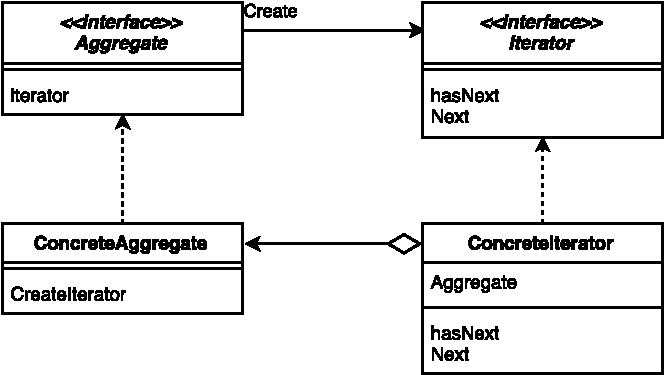
\includegraphics[width=0.7\textwidth]{IteratorPatan-crop.pdf}
			\caption{(例)Iteratorパターン}\label{fig::iterator}
		\end{figure}
		
	\subsection{私見}
		C++のIteratorと同じようなものかと思ったが、それは今回のパターンとは少し実装の仕方が違っている気がした。
		特にC++はインターフェイスを使っておらず、Iteratorクラスの定義が、Aggregateクラスの中に書かれていた覚えがある。
		C\#のIEnumerableとIEnumeratorがこのパターンを使っているのだろうと感じた。
		
		自分でこのパターンを使ったこともあったが、
		その時はインターフェイスを作らずに直接Iteratorクラスを作ってしまった。
		その結果、Iteratorクラスの内容はかなり独特なものになってしまったと思う。
		インターフェイスを用いた方が、例でいうConcreteクラスの内容がどうであれインターフェイスの
		様式\footnote{今回の例ではhasNext、nextのメソッドを知っているだけで使える}
		のみを知っていれば扱えるようになるのがかなりのメリットだと感じた。
	\section{2018年3月30日時点のコメント}
		\subsection{感想}
			レポートを書こうと思い立って1日目が終了。
			
			\TeX の環境を構築したり、クラス図を作るための手段を調べるのに時間がかかってしまい、
			今回は1つのデザインパターンしか書けなかったが今後はもう少し早いペースで書いていけると思う。
			
			Iteratorパターンも読み始める前はわかっているつもりだったが、読んでみるとなかなか有益だったと思う。
		\subsection{疑問点}
			現在のところ特になし。
			\clearpage
			
			
			
			
			
			
			
			
			
			
			
			
			
			
			
			
			
			
			
			
			
			
			
			
			
			
			
			
			
			
			
			
			
			
			
		
\end{document}